\section{Importance of Numerical Stability in Survival Models}

Numerical stability is a critical yet often overlooked aspect of implementing survival models, particularly those based on parametric distributions and deep learning approaches \parencite{goldberg1991,hanin2022}. This chapter explores the numerical challenges that arise when implementing models like DSM \parencite{nagpal2021dsm} and MENSA \parencite{zhong2021}, and provides practical solutions to ensure robustness and reliability.

\begin{notebox}[title=Chapter Overview]
This chapter covers:
\begin{itemize}
    \item Common numerical challenges in parametric survival models
    \item Critical calculations prone to instability
    \item Practical techniques for ensuring numerical stability
    \item Implementation strategies for robust survival models
    \item Testing approaches to verify numerical reliability
    \item The broader importance of stability for model deployment
\end{itemize}
\end{notebox}

Parametric survival models are particularly sensitive to numerical issues due to the complex mathematical forms of their distribution functions and the wide range of time scales they must handle. Small errors in calculation can lead to training failure, model divergence, or unreliable predictions. Achieving stability requires balancing precision with computational efficiency and implementing safeguards against various numerical pitfalls.

\section{Common Numerical Challenges}

Implementation of survival models faces several fundamental numerical challenges that can undermine model performance and reliability.

\subsection{Underflow and Overflow}

Floating-point arithmetic has inherent limitations in representing very small or very large numbers, leading to two common issues:

\begin{definitionbox}[title=Underflow and Overflow]
\begin{itemize}
    \item \textbf{Underflow:} Occurs when a value becomes too small to be represented in the floating-point format, resulting in it being rounded to zero.
    \begin{itemize}
        \item Example: $S(t) \approx 0$ for large $t$ values
        \item Problem: $\log(S(t))$ becomes $-\infty$
        \item Occurs when values are smaller than minimum representable float ($\approx 10^{-38}$ for float32)
    \end{itemize}

    \item \textbf{Overflow:} Occurs when a value becomes too large to be represented, resulting in it being set to infinity.
    \begin{itemize}
        \item Example: $e^x$ for $x > 709$ in float64
        \item Problem: Large intermediate calculations explode to infinity
        \item Produces infinity or NaN values that corrupt subsequent computations
    \end{itemize}
\end{itemize}
\end{definitionbox}

These issues are particularly relevant in survival analysis where we often calculate probabilities that can be extremely small (e.g., survival probability beyond a certain point) or use exponential functions that can grow extremely large.

\begin{figure}[htbp]
    \centering
    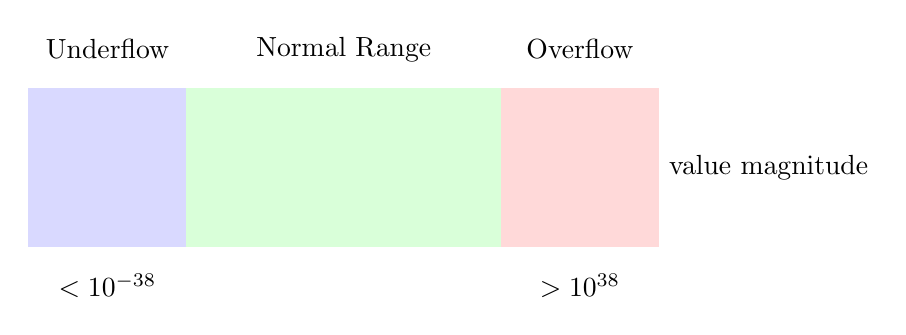
\begin{tikzpicture}
        \draw[->,thick] (0,2) -- (8,2) node[right] {value magnitude};

        % Underflow region
        \filldraw[blue!15] (0,1) rectangle (2,3);
        \node at (1,3.5) {Underflow};
        \node at (1,0.5) {$< 10^{-38}$};

        % Normal region
        \filldraw[green!15] (2,1) rectangle (6,3);
        \node at (4,3.5) {Normal Range};

        % Overflow region
        \filldraw[red!15] (6,1) rectangle (8,3);
        \node at (7,3.5) {Overflow};
        \node at (7,0.5) {$> 10^{38}$};
    \end{tikzpicture}
    \caption{Floating-point representation ranges for 32-bit floats. Values outside the normal range suffer from underflow or overflow, leading to precision loss or invalid operations.}
    \label{fig:float-ranges}
\end{figure}

\subsection{Precision Loss and Invalid Operations}

Beyond underflow and overflow, other numerical issues can compromise calculation integrity:

\begin{itemize}
    \item \textbf{Catastrophic cancellation:} Loss of significant digits when subtracting two nearly equal numbers.
    \begin{itemize}
        \item Example: Computing $1 - S(t)$ when $S(t) \approx 1$
        \item Problem: Significant digits lost in close subtractions
        \item Critical for cumulative distribution: $F(t) = 1 - S(t)$
    \end{itemize}

    \item \textbf{NaN propagation:} When an invalid operation occurs (e.g., division by zero, log of negative number), it produces a "Not a Number" (NaN) value that contaminates all subsequent calculations.
    \begin{itemize}
        \item Example: $\log(0)$ or $\sqrt{-1}$ in computation
        \item Problem: NaN infects all subsequent calculations
        \item Particularly damaging in backward pass (autograd)
    \end{itemize}
\end{itemize}

\begin{examplebox}[title=Catastrophic Cancellation Example]
Consider computing $1 - 0.999999$ with limited precision:
\begin{itemize}
    \item With full precision: $1.000000 - 0.999999 = 0.000001$ (correct)
    \item With 7 digits precision: $1.0 - 0.999999 \approx 0.0$ (incorrect)
\end{itemize}
This type of error is especially problematic when computing the cumulative distribution function $F(t) = 1 - S(t)$ for small values of $t$ where $S(t)$ is very close to 1.
\end{examplebox}

\section{Critical Calculations in Survival Models}

Certain calculations in survival models are particularly prone to numerical instability and require special attention.

\subsection{Hazard Function Calculations}

The hazard function, defined as $h(t) = \frac{f(t)}{S(t)}$, is a common source of numerical issues:

\begin{itemize}
    \item Division by very small $S(t)$ at large $t$ can cause overflow
    \item For Weibull distribution: $h(t) = \frac{\alpha}{\lambda}\left(\frac{t}{\lambda}\right)^{\alpha-1}$
    \item Two problematic regions:
    \begin{itemize}
        \item Large $t$: $S(t) \approx 0$ causing division by near-zero
        \item Small $t$ with $\alpha < 1$: Negative exponent causes explosion as $t$ approaches zero
    \end{itemize}
\end{itemize}

\begin{figure}[htbp]
    \centering
    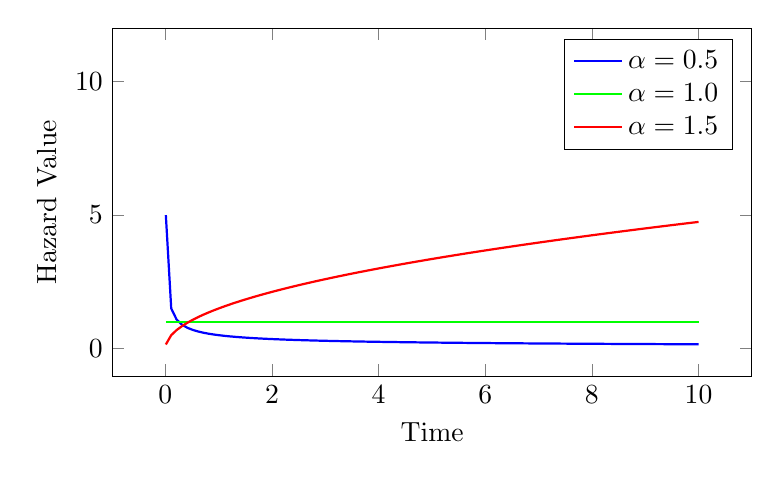
\begin{tikzpicture}
        \begin{axis}[
            width=0.8\textwidth,
            height=6cm,
            xlabel={Time},
            ylabel={Hazard Value},
            domain=0.01:10,
            samples=100,
            ymax=12,
            legend pos=north east,
          ]

          % Weibull hazard with alpha < 1
          \addplot[blue, thick] {0.5*x^(-0.5)};

          % Weibull hazard with alpha = 1
          \addplot[green, thick] {1};

          % Weibull hazard with alpha > 1
          \addplot[red, thick] {1.5*x^0.5};

          \legend{$\alpha = 0.5$, $\alpha = 1.0$, $\alpha = 1.5$}
        \end{axis}
    \end{tikzpicture}
    \caption{Weibull hazard functions with different shape parameters. When $\alpha < 1$ (blue), the hazard explodes as $t$ approaches zero, creating numerical instability.}
    \label{fig:weibull-hazards}
\end{figure}

\begin{examplebox}[title=Weibull Hazard Calculation Issues]
For a Weibull distribution with $\alpha = 0.5$ and $\lambda = 1$:
\begin{center}
    \begin{tabular}{|c|c|}
        \hline
        \textbf{Time} & \textbf{Hazard Value} \\
        \hline
        0.001 & 15.8 \\
        0.01 & 5.0 \\
        0.1 & 1.6 \\
        1.0 & 0.5 \\
        10.0 & 0.16 \\
        \hline
    \end{tabular}
\end{center}

As $t$ approaches zero, the hazard value explodes due to the negative exponent ($\alpha-1 = -0.5$). This can cause:
\begin{itemize}
    \item Overflow in hazard value computation
    \item Unstable gradients during backpropagation
    \item Cascade of NaN values in forward/backward passes
    \item Training failure without proper safeguards
\end{itemize}
\end{examplebox}

\subsection{Mixture Model Challenges}

Mixture models like DSM face additional numerical challenges:

\begin{itemize}
    \item \textbf{Mixture log-likelihood:} Computing $\log \sum_k \pi_k f_k(t)$ can be unstable
    \begin{itemize}
        \item Underflow if all $f_k(t)$ are very small
        \item Sum becomes effectively zero, leading to $\log(0) = -\infty$
        \item Common for points in tails of all components
    \end{itemize}

    \item \textbf{Component scale disparity:} Component densities can span many orders of magnitude
    \begin{itemize}
        \item Some components contribute negligibly
        \item Numeric precision lost in summation
        \item Gradient flow dominated by the largest components
    \end{itemize}
\end{itemize}

\begin{figure}[htbp]
    \centering
    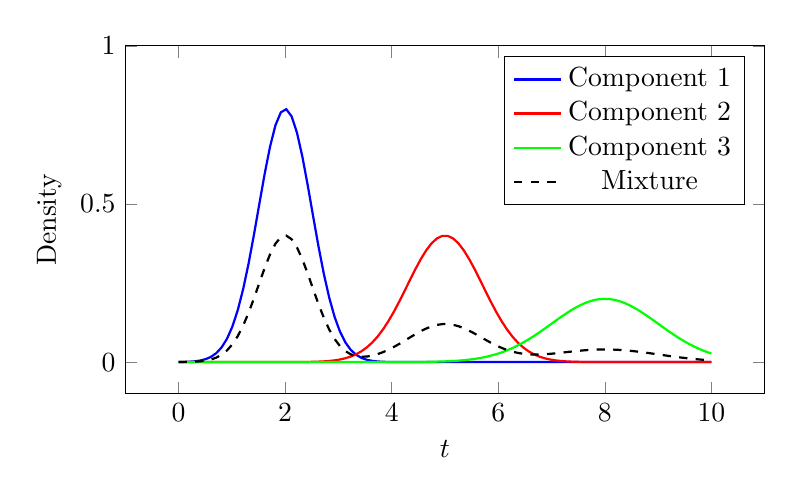
\begin{tikzpicture}
        \begin{axis}[
            width=0.8\textwidth,
            height=6cm,
            xlabel={$t$},
            ylabel={Density},
            domain=0:10,
            samples=100,
            ymax=1,
            legend pos=north east,
          ]

          % Component densities
          \addplot[blue, thick] {0.8*exp(-(x-2)^2/0.5)};
          \addplot[red, thick] {0.4*exp(-(x-5)^2/1)};
          \addplot[green, thick] {0.2*exp(-(x-8)^2/2)};

          % Mixture density
          \addplot[black, thick, dashed] {0.5*0.8*exp(-(x-2)^2/0.5) + 0.3*0.4*exp(-(x-5)^2/1) + 0.2*0.2*exp(-(x-8)^2/2)};

          \legend{Component 1, Component 2, Component 3, Mixture}
        \end{axis}
    \end{tikzpicture}
    \caption{A mixture model combines multiple component distributions. Near the tails, some components' densities can be orders of magnitude smaller than others, leading to numerical challenges.}
    \label{fig:mixture-densities}
\end{figure}

\subsection{Gradient Computation Challenges}

Automatic differentiation in deep learning frameworks produces gradients that can also suffer from numerical instability:

\begin{itemize}
    \item \textbf{Backpropagation through exponentiation:}
    \begin{itemize}
        \item Gradient of $e^x$ is $e^x$
        \item For large $x$, gradient explodes
        \item For very negative $x$, gradient vanishes
        \item Example: $x = 100 \Rightarrow e^x \approx 10^{43} \Rightarrow \nabla_x e^x \approx 10^{43}$
    \end{itemize}

    \item \textbf{Weibull-specific gradient issues:}
    \begin{itemize}
        \item Shape parameter gradient scales with time values
        \item Can lead to instability with diverse time ranges
        \item Extreme parameter values exacerbate gradient issues
    \end{itemize}

    \item \textbf{NaN propagation in gradients:}
    \begin{itemize}
        \item One invalid operation can corrupt the entire backward pass
        \item Requires comprehensive guarding throughout computation
        \item Affects all model parameters, not just the problematic ones
    \end{itemize}
\end{itemize}

\begin{figure}[htbp]
    \centering
    \begin{tikzpicture}
        % Forward computation
        \node[draw, rounded corners, fill=blue!10, minimum width=3cm, minimum height=0.8cm] (input) at (0,0) {Parameter Inputs};
        \node[draw, rounded corners, fill=blue!10, minimum width=3cm, minimum height=0.8cm] (forward) at (0,-1.5) {Forward Computation};
        \node[draw, rounded corners, fill=blue!10, minimum width=3cm, minimum height=0.8cm] (loss) at (0,-3) {Loss Value};

        % Backward computation (gradient)
        \node[draw, rounded corners, fill=red!10, minimum width=3cm, minimum height=0.8cm] (dloss) at (5,-3) {$\nabla$ Loss};
        \node[draw, rounded corners, fill=red!10, minimum width=3cm, minimum height=0.8cm] (dforward) at (5,-1.5) {$\nabla$ Computation};
        \node[draw, rounded corners, fill=red!10, minimum width=3cm, minimum height=0.8cm] (dparam) at (5,0) {$\nabla$ Parameters};

        % NaN contamination
        \node[draw, star, fill=yellow, inner sep=1pt] at (5,-1.5) {};
        \node[text width=3cm] at (8,-1.5) {NaN generated here};

        % Connect nodes
        \draw[->, thick] (input) -- (forward);
        \draw[->, thick] (forward) -- (loss);
        \draw[->, thick] (loss) -- (dloss);
        \draw[->, thick] (dloss) -- (dforward);
        \draw[->, thick, red, dashed] (dforward) -- (dparam) node[midway, right] {NaN propagation};

        % Draw x through whole gradient path to indicate corruption
        \draw[red, thick, line width=1pt] (3.5,-3.5) -- (6.5,0.5);
        \draw[red, thick, line width=1pt] (3.5,0.5) -- (6.5,-3.5);
    \end{tikzpicture}
    \caption{NaN propagation in the backward pass: a single numerical error in gradient computation propagates and corrupts all parameter updates.}
    \label{fig:nan-gradient-propagation}
\end{figure}

\section{Solutions for Numerical Stability}

Several proven techniques can address these numerical challenges and ensure stable model implementation.

\subsection{Log-Domain Calculations}

Working in the logarithmic domain is perhaps the most important technique for preventing underflow and overflow:

\begin{equationbox}[title=Log-Domain Transformations]
Instead of computing $S(t)$ directly, compute $\log S(t)$ and only exponentiate when necessary:
\begin{align}
    \log S(t) &= -\left(\frac{t}{\lambda}\right)^{\alpha} \\
    S(t) &= \exp\left(\log S(t)\right)
\end{align}

Key transformations:
\begin{align}
    \log(a \cdot b \cdot c) &= \log(a) + \log(b) + \log(c) \\
    \log\left(\frac{a}{b}\right) &= \log(a) - \log(b) \\
    \log(a^b) &= b \cdot \log(a)
\end{align}
\end{equationbox}

\begin{examplebox}[title=Log-Domain Calculation Examples]
Common survival calculations in log-domain:
\begin{center}
    \begin{tabular}{|l|l|}
        \hline
        \textbf{Standard Form} & \textbf{Log-Domain Form} \\
        \hline
        $S(t) = \exp(-(\frac{t}{\lambda})^{\alpha})$ & $\log S(t) = -(\frac{t}{\lambda})^{\alpha}$ \\
        \hline
        $f(t) = \frac{\alpha}{\lambda}(\frac{t}{\lambda})^{\alpha-1}S(t)$ & $\log f(t) = \log(\frac{\alpha}{\lambda}) + (\alpha-1)\log(\frac{t}{\lambda}) + \log S(t)$ \\
        \hline
    \end{tabular}
\end{center}

Value ranges comparison:
\begin{center}
    \begin{tabular}{|c|c|c|}
        \hline
        \textbf{x} & \textbf{$e^x$} & \textbf{$\log y$} \\
        \hline
        -10 & 0.00005 & -10 \\
        -1 & 0.368 & -1 \\
        0 & 1 & 0 \\
        1 & 2.718 & 1 \\
        10 & 22026 & 10 \\
        100 & $\approx 10^{43}$ & 100 \\
        710 & \textcolor{red}{OVERFLOW} & 710 \\
        \hline
    \end{tabular}
\end{center}

Working in log-domain keeps values in a numerically stable range, even for extremely large or small inputs.
\end{examplebox}

\subsection{Log-Sum-Exp Trick}

The log-sum-exp trick is crucial for stable computation of mixture models:

\begin{equationbox}[title=Log-Sum-Exp Trick]
For stable computation of $\log \sum_i e^{x_i}$:
\begin{align}
    \log \sum_i e^{x_i} &= \log \left[ e^a \sum_i e^{x_i - a}\right] \\
    &= a + \log \sum_i e^{x_i - a}
\end{align}
where $a = \max_i x_i$

This technique subtracts the maximum value before exponentiation, preventing overflow while maintaining mathematical equivalence.
\end{equationbox}

\begin{figure}[htbp]
    \centering
    \begin{tikzpicture}
        \draw[->,thick] (0,0) -- (8,0) node[right] {$z$};
        \draw[->,thick] (0,0) -- (0,4) node[above] {$e^z$};

        % Original values
        \filldraw[blue] (1,0.1) circle (2pt) node[below] {$z_1$};
        \filldraw[blue] (3,0.1) circle (2pt) node[below] {$z_2$};
        \filldraw[blue] (6,0.1) circle (2pt) node[below] {$z_3 = a$};

        % Exponential curve
        \draw[domain=0:6.2,smooth,variable=\x,blue] plot ({\x},{0.2*exp(\x-1)});

        % Shifted values
        \filldraw[red] (1,0.1) circle (2pt) node[above left] {$z_1-a$};
        \filldraw[red] (3,0.1) circle (2pt) node[above left] {$z_2-a$};
        \filldraw[red] (6,0.1) circle (2pt) node[above left] {$z_3-a=0$};

        % Shifted exponential (manageable values)
        \draw[domain=0:6.2,smooth,variable=\x,red] plot ({\x},{0.2*exp(\x-6)});

        \node[text width=4cm] at (4,3) {Shifting by max value keeps exponentials manageable};
    \end{tikzpicture}
    \caption{The log-sum-exp trick: By subtracting the maximum value before exponentiation, all values in the exponential become $\leq 1$, preventing overflow while maintaining mathematical equivalence.}
    \label{fig:log-sum-exp}
\end{figure}

Implementation process:
\begin{enumerate}
    \item Find maximum value $a = \max_k z_k$
    \item Subtract $a$ from each $z_k$ before exponentiation
    \item Sum the resulting values (all $\leq 1$)
    \item Take logarithm and add $a$ back
\end{enumerate}

Key benefits:
\begin{itemize}
    \item Prevents underflow in the sum
    \item Works even when components span many orders of magnitude
    \item Preserves numerical precision
    \item Mathematically equivalent to direct computation
    \item Critical for mixture model stability
\end{itemize}

\subsection{Gradient Detachment Strategy}

Safe gradient computation is essential for stable training. Standard techniques like gradient clipping may not be sufficient for the extreme cases encountered in survival models.

\begin{notebox}[title=Gradient Challenges]
Problems with standard operations:
\begin{itemize}
    \item NaN gradients stop backward propagation entirely
    \item Boolean masking requires shape compatibility
    \item Clipping alone doesn't fix fundamental gradient issues
    \item Safe paths are needed for extreme input regions
\end{itemize}
\end{notebox}

The gradient detachment approach provides a robust solution:

\begin{equationbox}[title=Gradient Detachment With Safe Masking]
\begin{align}
    \text{unsafe\_mask} &= (x > \text{threshold}).float() \\
    \text{safe\_mask} &= 1.0 - \text{unsafe\_mask} \\
    \text{normal\_result} &= \text{original\_function}(x) \\
    \text{fallback} &= \text{safe\_value} \\
    \text{result} &= \text{safe\_mask} \cdot \text{normal\_result} + \text{unsafe\_mask} \cdot \text{fallback}
\end{align}

This approach:
\begin{itemize}
    \item Prevents NaN propagation while allowing normal calculation in safe regions
    \item Enables training to continue despite some extreme values
    \item Creates smooth transitions between computation regimes
    \item Maintains gradient flow through valid components
\end{itemize}
\end{equationbox}

\begin{figure}[htbp]
    \centering
    \begin{tikzpicture}
        % Visualization of the safe masking approach
        % Input and branches
        \node[draw, circle, fill=blue!10, minimum size=1cm] (input) at (0,0) {Input};

        % Two computation paths
        \node[draw, ellipse, fill=green!10, minimum width=2cm, minimum height=1cm] (normal) at (-1.5,-2) {Normal Path};
        \node[draw, ellipse, fill=yellow!10, minimum width=2cm, minimum height=1cm] (fallback) at (1.5,-2) {Fallback Path};

        % Masks
        \node[draw, ellipse, fill=blue!10, minimum width=1.5cm, minimum height=0.8cm] (safe) at (-2.5,-0.8) {Safe Mask};
        \node[draw, ellipse, fill=blue!10, minimum width=1.5cm, minimum height=0.8cm] (unsafe) at (2.5,-0.8) {Unsafe Mask};

        % Output combination
        \node[draw, ellipse, fill=blue!10, minimum width=2cm, minimum height=1cm] (output) at (0,-4) {Combined Result};

        % Arrows
        \draw[->, thick] (input) -- (normal);
        \draw[->, thick] (input) -- (fallback);
        \draw[->, thick] (input) -- (safe);
        \draw[->, thick] (input) -- (unsafe);
        \draw[->, thick] (normal) -- node[left] {$\times$} (output);
        \draw[->, thick] (fallback) -- node[right] {$\times$} (output);
        \draw[->, thick, dashed] (safe) -- (-1.5,-3);
        \draw[->, thick, dashed] (unsafe) -- (1.5,-3);

        % Formula at bottom
        \node[text width=6cm, align=center] at (0,-5) {result = safe\_mask $\times$ normal\_result + unsafe\_mask $\times$ fallback};
    \end{tikzpicture}
    \caption{Gradient detachment with safe masking: Input values are classified into safe and unsafe regions, with a separate computation path for each, then combined using masks to ensure stability.}
    \label{fig:gradient-detachment}
\end{figure}

\subsection{Case Study: Weibull Hazard Stabilization}

Weibull hazard calculation is particularly challenging when the shape parameter $\alpha < 1$, causing the hazard to approach infinity as $t \rightarrow 0$:

\begin{align}
    h(t) = \frac{\alpha}{\lambda}\left(\frac{t}{\lambda}\right)^{\alpha-1}
\end{align}

Special handling required:
\begin{itemize}
    \item Log-domain computation always
    \item Special clamping near $t=0$
    \item Shape parameter buffer ($\alpha > 0.05$)
\end{itemize}

Implementation approaches:
\begin{itemize}
    \item Clamping shape-1 to prevent extreme negative exponents:
    \begin{align}
        \text{shape\_m1} &= \text{clamp(shape - 1.0, min=-0.95)}
    \end{align}
    \item Using log domain to compute power terms:
    \begin{align}
        \text{log\_power} &= \text{shape\_m1} \cdot \text{log\_ratio} \\
        \text{power} &= \text{exp(log\_power)}
    \end{align}
\end{itemize}

These approaches ensure safe computation even for small $t$ values and shape parameters less than 1, maintaining the same values in safe regions while preventing overflow in extreme regions.

\section{Loss Function Stability Techniques}

Beyond individual calculations, ensuring the overall loss function is numerically stable is crucial for reliable training.

\subsection{NaN Detection and Reporting}

Early detection of numerical issues helps identify and address problems:

\begin{itemize}
    \item Implement NaN detection in the loss computation:
    \begin{verbatim}
    if debug_nans and torch.isnan(log_likelihood).any():
        print(f"NaN detected: {torch.isnan(log_likelihood).sum().item()}")
    \end{verbatim}
    \item Provides early warning during training
    \item Helps identify specific components causing issues
    \item Can be conditionally enabled during development
\end{itemize}

\subsection{Safe Loss Aggregation}

When computing losses over multiple samples or components, handle invalid values gracefully:

\begin{itemize}
    \item Skip invalid components when aggregating losses:
    \begin{verbatim}
    # Only add valid losses
    if torch.isfinite(event_loss):
        total_loss = total_loss + event_loss
        total_valid_events += 1
    \end{verbatim}
    \item Prevents a single invalid value from corrupting the entire batch
    \item Maintains gradient flow through valid samples
    \item Allows training to continue despite some problematic data points
\end{itemize}

\subsection{Fallback Mechanism}

As a last resort, implement a fallback for the overall loss:

\begin{itemize}
    \item Provide a safety net for extreme cases:
    \begin{verbatim}
    if not torch.isfinite(final_loss):
        logger.warning(f"Non-finite loss: {final_loss.item()}")
        final_loss = torch.tensor(1.0, device=device, requires_grad=True)
    \end{verbatim}
    \item Allows training to continue despite some invalid values
    \item Prevents entire training run from failing due to occasional issues
    \item Logs warnings to alert developers about the problem
    \item Should be a rare occurrence in a well-designed model
\end{itemize}

\section{Testing for Numerical Stability}

Comprehensive testing is essential to verify numerical stability across a wide range of inputs and conditions.

\subsection{Extreme Value Testing}

Test models with input values at the extremes of expected ranges:

\begin{itemize}
    \item \textbf{Very small/large time values:}
    \begin{itemize}
        \item Test with $t \approx 0$ (e.g., $10^{-10}$)
        \item Test with very large $t$ (e.g., $10^{10}$)
        \item Check edge cases where $S(t) \approx 0$ or $S(t) \approx 1$
    \end{itemize}

    \item \textbf{Boundary shape parameters:}
    \begin{itemize}
        \item Test with $\alpha$ very close to 0 (e.g., 0.01)
        \item Test with $\alpha$ near 1.0 (important transition point)
        \item Test with very large $\alpha$ values (e.g., 20+)
    \end{itemize}
\end{itemize}

\subsection{Gradient Testing}

Explicitly test the backward pass to ensure stable gradient computation:

\begin{itemize}
    \item \textbf{Test backward pass explicitly:}
    \begin{itemize}
        \item Verify gradient computation with torch.autograd.grad()
        \item Ensure gradients are finite for all parameters
        \item Compare analytical vs. numerical gradients
    \end{itemize}

    \item \textbf{Gradient monitoring during training:}
    \begin{itemize}
        \item Track gradient norms over training epochs
        \item Detect sudden spikes in gradient magnitude
        \item Implement gradient clipping as safety mechanism
    \end{itemize}
\end{itemize}

\subsection{Comprehensive Test Coverage}

Ensure test coverage across all critical aspects of the model:

\begin{itemize}
    \item Input values across the full range of time scales
    \item All parameter ranges, especially near boundaries
    \item Gradient flow through all model components
    \item Mixture models with various component configurations
    \item Censored and uncensored data points
    \item Edge cases specific to your application domain
\end{itemize}

\begin{figure}[htbp]
    \centering
    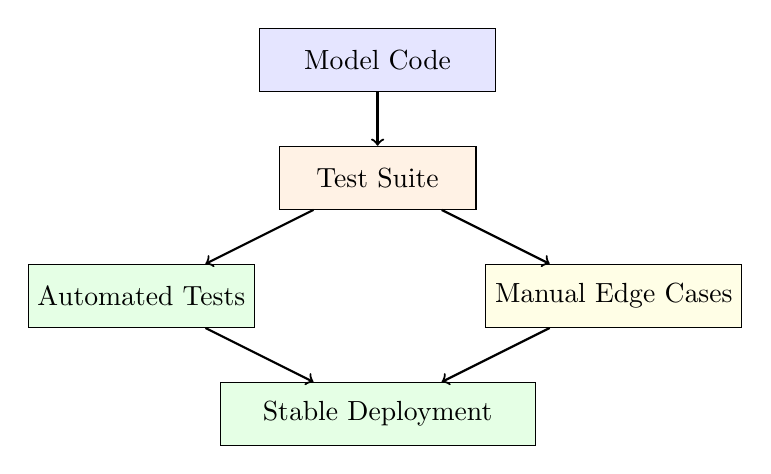
\begin{tikzpicture}
        % Create a test pipeline visualization
        \node[draw, rectangle, fill=blue!10, minimum width=3cm, minimum height=0.8cm] (code) at (0,0) {Model Code};

        \node[draw, rectangle, fill=orange!10, minimum width=2.5cm, minimum height=0.8cm] (tests) at (0,-1.5) {Test Suite};

        \node[draw, rectangle, fill=green!10, minimum width=2.8cm, minimum height=0.8cm] (auto) at (-3,-3) {Automated Tests};
        \node[draw, rectangle, fill=yellow!10, minimum width=2.8cm, minimum height=0.8cm] (manual) at (3,-3) {Manual Edge Cases};

        \node[draw, rectangle, fill=green!10, minimum width=4cm, minimum height=0.8cm] (deploy) at (0,-4.5) {Stable Deployment};

        % Connect nodes
        \draw[->, thick] (code) -- (tests);
        \draw[->, thick] (tests) -- (auto);
        \draw[->, thick] (tests) -- (manual);
        \draw[->, thick] (auto) -- (deploy);
        \draw[->, thick] (manual) -- (deploy);
    \end{tikzpicture}
    \caption{A comprehensive testing pipeline for ensuring numerical stability, combining automated tests with manual verification of edge cases.}
    \label{fig:testing-pipeline}
\end{figure}

\section{The Importance of Numerical Stability for Deployment}

Numerical stability is not merely a technical detail—it forms the foundation for reliable model deployment in real-world applications.

\subsection{Critical Applications}

In high-stakes domains like healthcare, numerical instability can have serious consequences:

\begin{itemize}
    \item Invalid predictions could lead to incorrect medical decisions
    \item Inconsistent model behavior undermines trust in the system
    \item Training failures delay model development and deployment
    \item Production issues may be difficult to diagnose and fix
\end{itemize}

\begin{figure}[htbp]
    \centering
    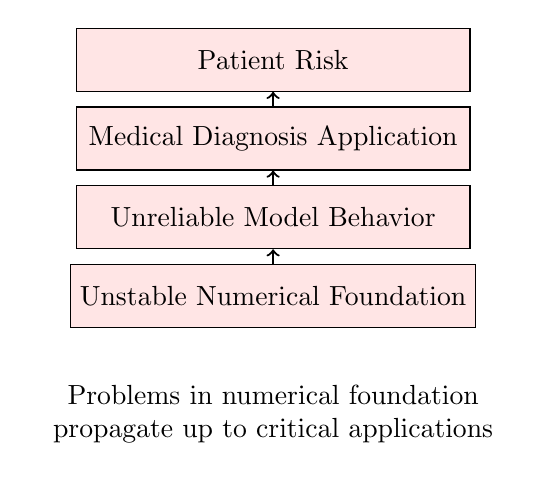
\begin{tikzpicture}
        % Critical applications stack
        \node[draw, rectangle, fill=red!10, minimum width=5cm, minimum height=0.8cm] (unstable) at (0,0) {Unstable Numerical Foundation};

        \node[draw, rectangle, fill=red!10, minimum width=5cm, minimum height=0.8cm] (model) at (0,1) {Unreliable Model Behavior};

        \node[draw, rectangle, fill=red!10, minimum width=5cm, minimum height=0.8cm] (application) at (0,2) {Medical Diagnosis Application};

        \node[draw, rectangle, fill=red!10, minimum width=5cm, minimum height=0.8cm] (risk) at (0,3) {Patient Risk};

        % Arrows connecting layers
        \draw[->, thick] (unstable) -- (model);
        \draw[->, thick] (model) -- (application);
        \draw[->, thick] (application) -- (risk);

        % Warning text
        \node[text width=6cm, align=center] at (0,-1.5) {Problems in numerical foundation propagate up to critical applications};
    \end{tikzpicture}
    \caption{The impact chain of numerical instability: Fundamental numerical issues propagate upward through the model to affect critical applications and ultimately patient outcomes.}
    \label{fig:stability-impact}
\end{figure}

\subsection{Technical Benefits}

Beyond preventing catastrophic failures, numerical stability offers several technical advantages:

\begin{itemize}
    \item Ensures consistent results across hardware platforms
    \item Allows models to generalize beyond the training data range
    \item Improves convergence properties during training
    \item Enables reliable uncertainty quantification
    \item Facilitates model interpretability and explanation
\end{itemize}

\begin{figure}[htbp]
    \centering
    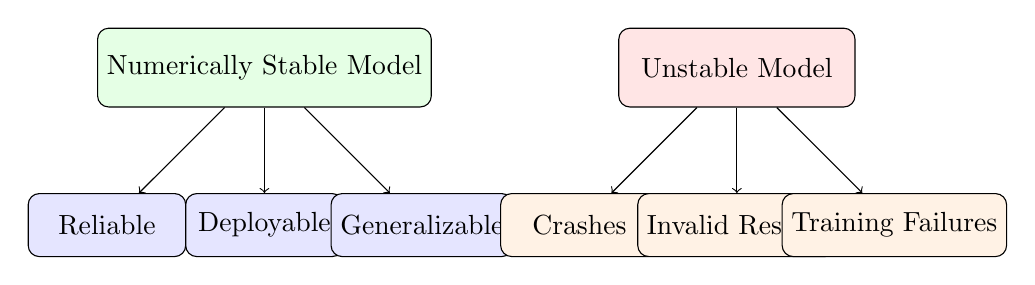
\begin{tikzpicture}
        % Stable vs unstable architecture diagram
        \node[draw, rounded corners, fill=green!10, minimum width=3cm, minimum height=1cm] (stable) at (0,0) {Numerically Stable Model};
        \node[draw, rounded corners, fill=red!10, minimum width=3cm, minimum height=1cm] (unstable) at (6,0) {Unstable Model};

        % Benefits of stable models
        \node[draw, rounded corners, fill=blue!10, minimum width=2cm, minimum height=0.8cm] (reliable) at (-2,-2) {Reliable};
        \node[draw, rounded corners, fill=blue!10, minimum width=2cm, minimum height=0.8cm] (deployable) at (0,-2) {Deployable};
        \node[draw, rounded corners, fill=blue!10, minimum width=2cm, minimum height=0.8cm] (generalizable) at (2,-2) {Generalizable};

        % Problems with unstable models
        \node[draw, rounded corners, fill=orange!10, minimum width=2cm, minimum height=0.8cm] (crashes) at (4,-2) {Crashes};
        \node[draw, rounded corners, fill=orange!10, minimum width=2cm, minimum height=0.8cm] (errors) at (6,-2) {Invalid Results};
        \node[draw, rounded corners, fill=orange!10, minimum width=2cm, minimum height=0.8cm] (training) at (8,-2) {Training Failures};

        % Connect nodes
        \draw[->] (stable) -- (reliable);
        \draw[->] (stable) -- (deployable);
        \draw[->] (stable) -- (generalizable);

        \draw[->] (unstable) -- (crashes);
        \draw[->] (unstable) -- (errors);
        \draw[->] (unstable) -- (training);
    \end{tikzpicture}
    \caption{Comparison of outcomes between numerically stable and unstable models. Stable models are reliable, deployable, and generalizable, while unstable models suffer from crashes, invalid results, and training failures.}
    \label{fig:stability-comparison}
\end{figure}

\section{Summary}

Numerical stability is a critical aspect of implementing parametric survival models, particularly deep learning approaches like DSM and MENSA. The key takeaways from this chapter include:

\begin{itemize}
    \item Underflow, overflow, and precision loss are common numerical challenges in survival models
    \item Hazard function calculations, mixture models, and gradient computation require special attention
    \item Working in the log domain, using the log-sum-exp trick, and implementing gradient detachment are effective solutions
    \item Loss function stability techniques, including NaN detection and safe aggregation, ensure reliable training
    \item Comprehensive testing across extreme values and boundary conditions is essential
    \item Numerical stability forms the foundation for reliable model deployment in critical applications
\end{itemize}

By implementing these techniques and remaining vigilant about numerical stability, we can build survival models that are not only theoretically sound but also practically reliable in real-world applications.

\begin{notebox}[title=Looking Ahead]
In the next chapter, we will explore how expert knowledge can be incorporated into survival models to enhance their performance and interpretability. This includes approaches for integrating domain expertise into model architecture, parameter constraints, and regularization strategies.
\end{notebox}
